En esta sección se va a explicar cómo se ha entrenado el modelo de detección de estado del pavimento. Comenzaremos explicando los parámetros de entrenamiento y otras consideraciones que se deben tener en cuenta a la hora de entrenar un modelo de detección de objetos. Después, se explicará cómo se han preparado los datos de la CRDDC2022 para tener en cuenta estas consideraciones y adaptar los datos a las particularidades de la librería Ultralytics. Por último, se explicará los requerimientos de hardware necesarios para entrenar los modelos de detección de objetos y cómo se ha llevado a cabo el entrenamiento en Google Colab durante el desarrollo de este TFG.

\subsection{Parámetros de entrenamiento y otras consideraciones}
Al entrenar modelos de aprendizaje profundo, se busca lograr una buena generalización, altas puntuaciones de precisión y recall, así como un entrenamiento rápido y eficiente. Para lograr estos objetivos se debe escoger cuidadosamente los parámetros de entrenamiento y tener en cuenta otras consideraciones clave.

La librería de Ultralytics proporciona una extensa lista de parámetros que se pueden ajustar para personalizar el entrenamiento de los modelos YOLO. La documentación de entrenamiento con Ultralytics YOLO \cite{ultralytics_train} incluye una lista de estos parámetros. En este TFG los parámetros más importantes que se han ajustado son el tamaño de modelo, el tamaño de batch, el número de épocas de entrenamiento, y la proporción de los datos anotados que se usa para entrenamiento y validación. A continuación, se explicará brevemente cada uno de estos parámetros y el efecto que tiene en el entrenamiento y rendimiento del modelo.

YOLOv8 tiene varios tamaños de modelo que se pueden usar. Los tamaños disponibles son \textit{nano}, \textit{small}, \textit{medium}, \textit{large} y \textit{very large}. Por lo general, para cualquier conjunto de datos, a mayor tamaño de modelo, mejor será la precisión del modelo y más latencia o tiempo de inferencia se necesitará. Además, a mayor tamaño de modelo, más memoria y tiempo de entrenamiento se necesitará. Por lo tanto, se debe elegir el tamaño de modelo que mejor se ajuste a las necesidades del proyecto. En la figura \ref{fig:yolo-comparison-plots}, extraída de la documentación de Ultralytics \cite{yolov8_ultralytics}, se puede ver una comparación de los tamaños de los modelos YOLO. Las gráficas muestran que YOLOv8 es la versión de YOLO con mejor mAP50-95 y que a mayor tamaño de modelo, mejor es la precisión del modelo. En la gráfica de la derecha se muestra que el tamaño de modelo también afecta negativamente a la velocidad de inferencia. El modelo \textit{nano} es el más rápido, pero también el menos preciso, mientras que el modelo \textit{very large} es el más preciso, pero también el más lento y el \textit{large} es el mejor equilibrio entre precisión y velocidad.

% Mostramos la graphs/yolo-comparison-plots.png
\begin{figure}[H]
    \centering
    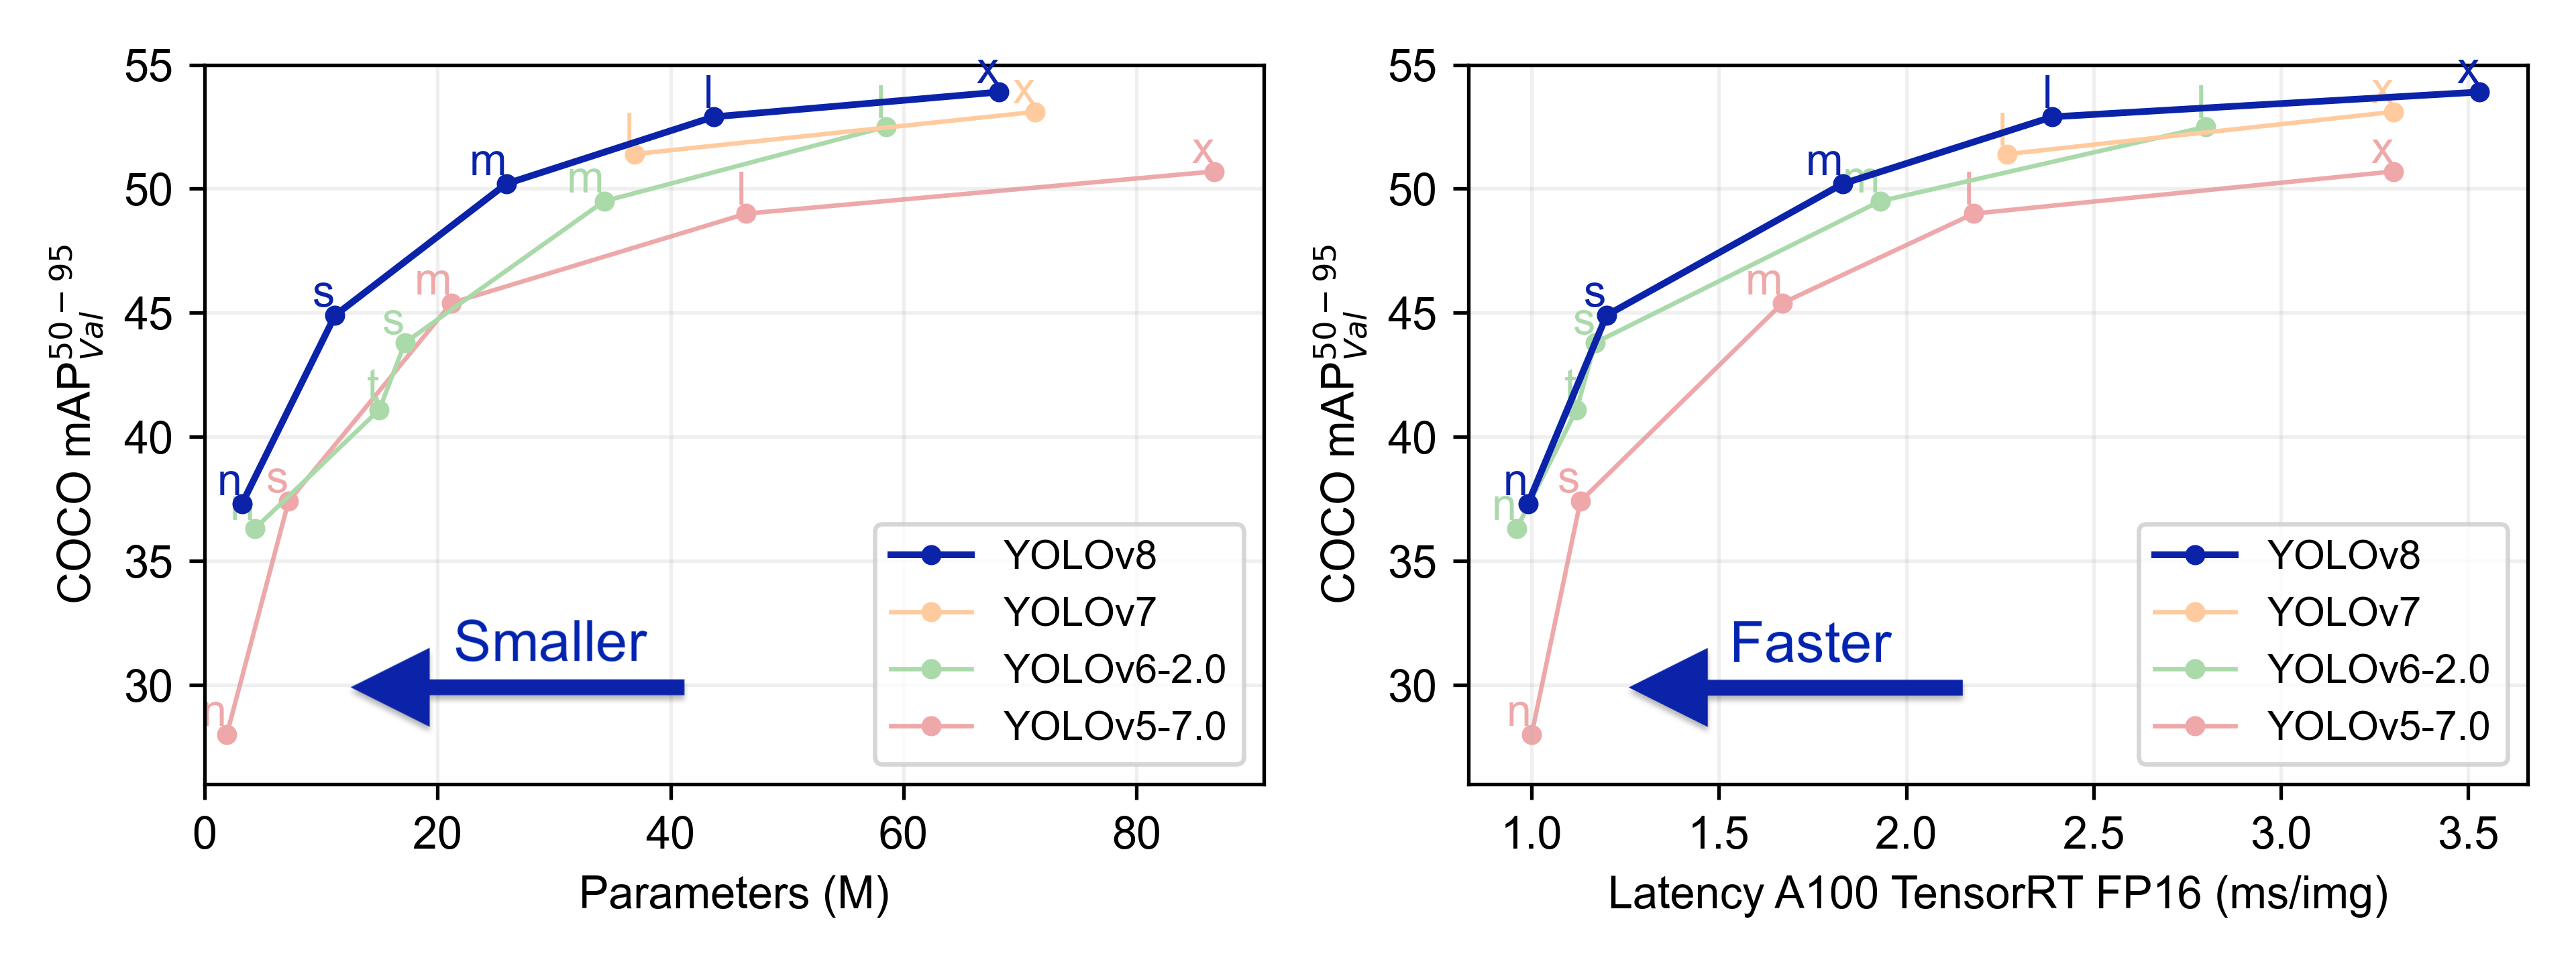
\includegraphics[width=1\textwidth]{graphs/yolo-comparison-plots.png}
    \caption{Comparación de los tamaños de los modelos YOLOv8 de Ultralytics. Figura extraída de \cite{ultralytics_yolov8_docs}.}
    \label{fig:yolo-comparison-plots}
\end{figure}

El número de épocas de entrenamiento y el tamaño de batch son dos hiperparámetros que determinan la cantidad de tiempo que se necesita para entrenar un modelo, la cantidad de memoria que se necesita y la velocidad de convergencia del modelo. Por lo general, a mayor número de épocas de entrenamiento, mejor será la precisión del modelo, pero también se corre el riesgo de sobreajustar el modelo al conjunto de entrenamiento. Por otro lado, a mayor tamaño de batch, más memoria se necesita, pero también se puede acelerar el entrenamiento. Por lo tanto, se debe elegir un número de épocas y un tamaño de batch que se ajuste a la capacidad de computación disponible. En el caso de los modelos de \textit{Computer Vision}, la capacidad de computación suele ser la limitación más importante, ya que los modelos de detección de objetos suelen ser muy grandes y necesitan mucha memoria y tiempo para entrenar.

El tamaño de batch se suele elegir en función de la capacidad de memoria de la GPU. Por lo general, se recomienda usar el tamaño de batch más grande que quepa en la memoria de la GPU para acelerar el entrenamiento. Sin embargo, si el tamaño de batch es demasiado grande, se puede producir un desbordamiento de memoria y el entrenamiento fallará. Un peligro de usar un tamaño de batch pequeño es que se generan estadísticas de normalización de lote (\textit{batch normalization statistics}) deficientes. Estas estadísticas son necesarias en el entrenamiento de modelos de aprendizaje profundo, ya que permiten normalizar los valores de las capas de la red neuronal y acelerar el entrenamiento. Si el tamaño de batch es demasiado pequeño, el rendimiento del modelo puede verse afectado negativamente y el entrenamiento puede ser más inestable, es decir, la pérdida puede oscilar más y el modelo puede tardar más en converger.

El número de épocas se puede fijar manualmente o se pueden aplicar criterios de parada temprana (\textit{early stopping}) para detener el entrenamiento cuando la pérdida en el conjunto de validación deja de disminuir. Este número es un hiperparámetro que se debe ajustar cuidadosamente, ya que un número de épocas demasiado bajo puede resultar en un modelo que no ha convergido, mientras que un número de épocas demasiado alto puede llevar a un modelo que se sobreajusta al conjunto de entrenamiento. Una forma de determinar si el número de épocas es adecuado es observar las curvas de pérdida en el conjunto de entrenamiento y en el conjunto de validación. Si la pérdida en el conjunto de validación comienza a aumentar mientras que la pérdida en el conjunto de entrenamiento sigue disminuyendo, es probable que el modelo se esté sobreajustando y se debe detener el entrenamiento.

En la figura \ref{fig:example_results} se muestra un ejemplo de los resultados de un modelo YOLOv8 de Ultralytics. En las curvas de pérdida de validación, \textit{val/box\_loss} y \textit{val/dfl\_loss}, se puede observar que el modelo se sobreajusta después de 90 épocas, ya que la pérdida en el conjunto de validación comienza a aumentar mientras que la pérdida en el conjunto de entrenamiento sigue disminuyendo.

% Añadir gráfica de example_results.png
\begin{figure}[H]
    \centering
    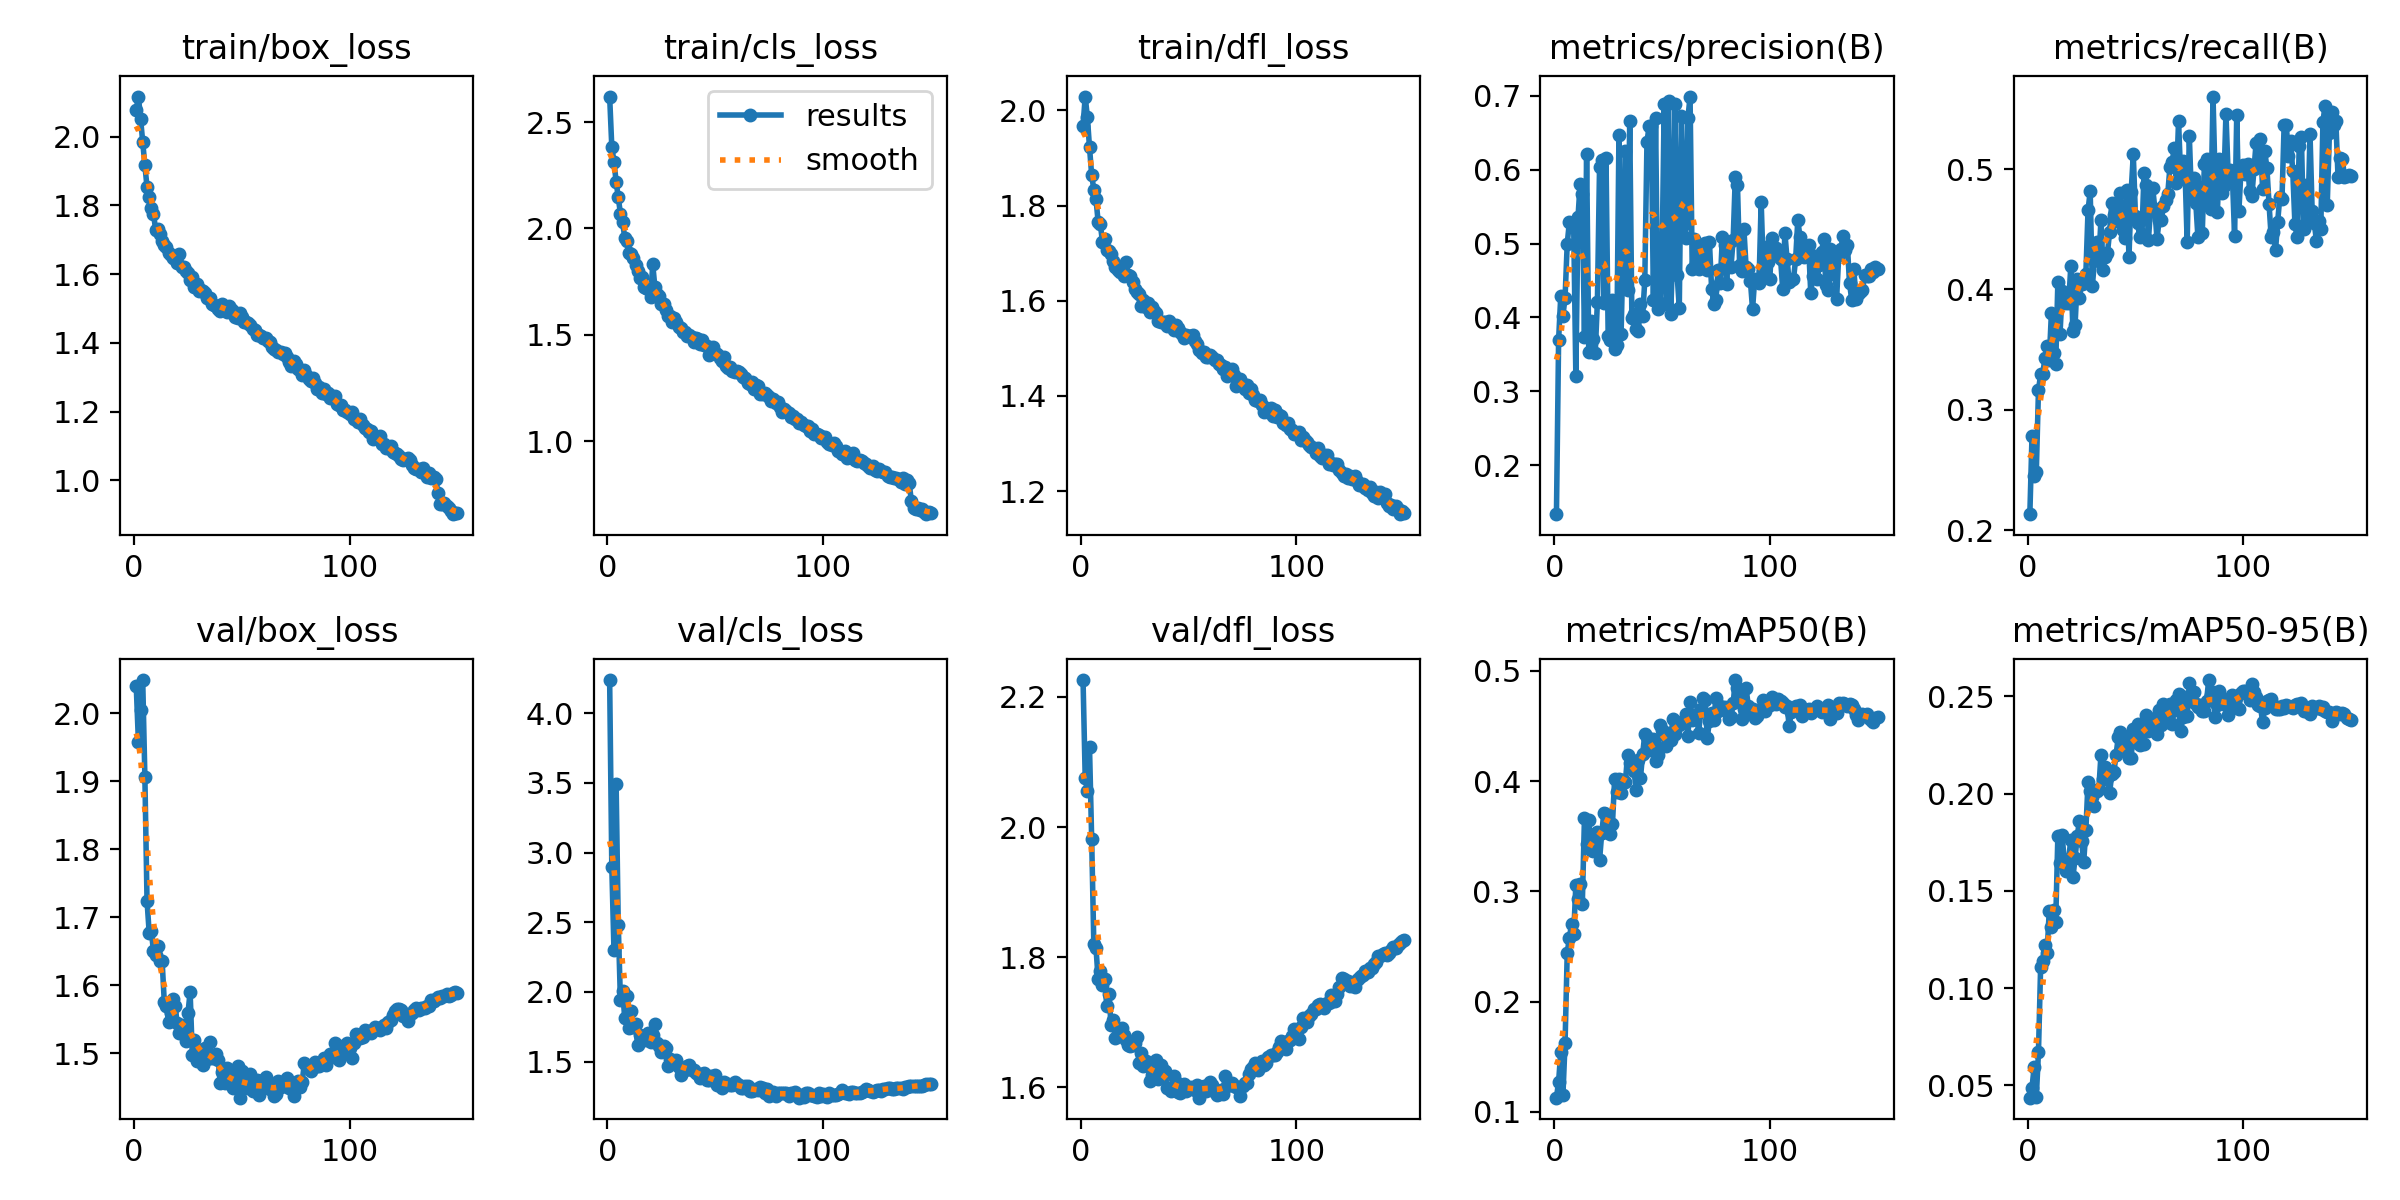
\includegraphics[width=0.9\textwidth]{graphs/example_results.png}
    \caption{Ejemplo de resultados de un modelo YOLOv8 de Ultralytics. En las curvas de perdida, box\_loss y dfl\_loss, se puede ver que el modelo se sobreajusta después de 90 épocas.}
    \label{fig:example_results}
\end{figure}

Como hemos visto en la figura \ref{fig:images_per_dataset_per_region}, la distribución de imágenes por región es muy desigual. Dependiendo de cómo se seleccione el conjunto de entrenamiento, esta diferencia en el número de imágenes por región puede afectar al rendimiento del modelo de diferentes maneras. Las tres estrategias más comunes son el \textit{undersampling}, \textit{oversampling} y no hacer nada.

El \textit{undersampling} consiste en seleccionar un número igual de imágenes de cada región, generalmente seleccionando tantas imágenes de cada región como la región con menos imágenes. El riesgo de esta técnica es que se pierde información de entrenamiento que podría ser útil para mejorar el modelo. Por otro lado, el \textit{oversampling} implica seleccionar múltiples veces las imágenes de los conjuntos con menos imágenes hasta tener tantas imágenes como el conjunto que más imágenes tiene. El riesgo de esta técnica es que puede llevar al sobreajuste a aquellas imágenes repetidas y además incrementa el tiempo de entrenamiento sin añadir información nueva. Sin embargo, tanto el \textit{undersampling} como el \textit{oversampling} solventan el problema de sobreajuste a las regiones con más imágenes.

La tercera estrategia es no hacer nada, lo que lleva a que el modelo se sobreajuste a las regiones con más imágenes. En este TFG se ha optado por esta tercera estrategia, ya que el \textit{undersampling} conllevaría una pérdida de información demasiado grande y el \textit{oversampling} aumentaría considerablemente el tiempo de ejecución, que ya es la limitación más grande en este TFG.

Una posible línea de trabajo futuro sería investigar si se puede mejorar el ajuste a los conjuntos de datos con menos imágenes mediante técnicas de \textit{data augmentation}, \textit{fine tuning} o incrementando el número de imágenes en estas regiones, por ejemplo, mediante Google Earth.


\subsection{Preparación de los datos}
En la sección de modelos [Sección \ref{SEC:MODELOS}] se ha explicado cómo se ha usado YOLO de Ultralytics para la detección del estado del pavimento. La elección de dicha librería nos obliga a realizar una serie de transformaciones en los datos para poder entrenar nuestros modelos. En esta subsección se va a explicar cómo se han preparado los datos de la CRDDC2022 para poder ser usados con YOLO de Ultralytics. Estos cambios se pueden encontrar detallados en los notebooks 'prepare-DatasetNinja.ipynb' y 'dataToYoloFormat.ipynb' en el repositorio del TFG \cite{TFG_Repository}.

Ultralytics requiere que las anotaciones tengan un formato específico para poder ser usadas en el entrenamiento de los modelos. En concreto, las anotaciones deben estar en un directorio llamado \texttt{labels} que esté en el mismo directorio que el directorio \texttt{images} que contiene las imágenes. Cada archivo de anotación debe tener el mismo nombre que el archivo de imagen correspondiente, pero con extensión '.txt' en lugar de '.jpg'. El contenido de cada archivo de anotación debe tener una línea por cada objeto en la imagen con el siguiente formato:
\begin{center}
    \texttt{<clase> <x> <y> <width> <height>}
\end{center}
Donde \texttt{<clase>} es el índice de la clase del objeto, \texttt{<x>} y \texttt{<y>} son las coordenadas del centro de la caja delimitadora normalizadas, y \texttt{<width>} y \texttt{<height>} son el ancho y el alto de la caja delimitadora normalizados. Las coordenadas normalizadas se calculan dividiendo las coordenadas de la caja delimitadora por el ancho y el alto de la imagen, respectivamente. Esta transformación se han realizado con el notebook 'prepare-DatasetNinja.ipynb' en el repositorio del TFG \cite{TFG_Repository}. Se han realizado otros cambios menos significativos como reducir el tamaño de las imágenes de Noruega para que sea más manejable en Google Colab.

\subsection{Entrenamiento en Google Colabs}
El entrenamiento de la mayoría de experimentos de este trabajo se han realizado en Google Colabs. Para ello, se ha desarrollado un notebook de Google Colabs llamado 'train-YOLOv8.ipynb' en el repositorio del TFG \cite{TFG_Repository}. Este notebook se encarga de instalar las dependencias necesarias, montar Google Drive para acceder a los datos y a los ficheros de configuración \textit{.yaml}, copiar los datos de Google Drive a la máquina virtual de Google Colabs, entrenar el modelo YOLOv8 con los datos y configuración proporcionados, y descargar los pesos del modelo entrenado a Google Drive. Adicionalmente, el notebook permite reanudar el entrenamiento de un modelo previamente entrenado. Este notebook lo ejecutaba en Google Colabs con una GPU Tesla T4, que es una GPU de gama media con 16 GB de memoria y 320 Turing Tensor Cores.


\subsection{Validación cruzada}
La validación es una parte fundamental en el desarrollo de modelos de aprendizaje automático, ya que permite comprobar si el modelo es capaz de generalizar bien a datos que no ha visto antes. La validación cruzada es una técnica que se utiliza para evaluar la capacidad de generalización de un modelo de aprendizaje automático. Consiste en dividir el conjunto de datos en $k$ subconjuntos, llamados \textit{folds}, y entrenar el modelo $k$ veces, cada vez utilizando un subconjunto distinto como conjunto de validación y el resto de subconjuntos como conjunto de entrenamiento. De esta forma, se obtienen $k$ métricas de evaluación distintas, una por cada iteración, y se pueden calcular métricas de evaluación globales como la media y la desviación estándar de las métricas de evaluación de cada iteración. En la figura \ref{fig:cross_validation} se puede ver un esquema de cómo se lleva a cabo la validación cruzada.

% Añadir la imagen K-fold_cross_validation.jpg de la carpeta img
\begin{figure}[H]
    \centering
    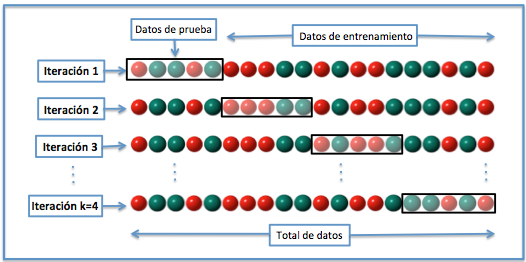
\includegraphics[width=0.9\textwidth]{img/K-fold_cross_validation.jpg}
    \caption{Esquema de validación cruzada. Figura extraída de \cite{KFoldCV_image}}
    \label{fig:cross_validation}
\end{figure}

En este TFG se ha llevado a cabo una validación cruzada de 4 \textit{folds} para evaluar los modelos. Es decir, cada iteración se ha entrenado con un 75\% de los datos anotados y se ha validado con el 25\% restante. Para dividir los datos se han separado las carpetas de \textit{train} de cada región en 4 subcarpetas \textit{fold\_0}, \textit{fold\_1}, \textit{fold\_2} y \textit{fold\_3}. Cada una de estas subcarpetas contiene un 25\% de las imágenes y anotaciones de la carpeta de \textit{train} correspondiente. De esta forma, cuando vamos a crear el fichero \textit{.yaml} que contiene la información de los datos de entrenamiento y validación, simplemente concatenamos las rutas de las subcarpetas \textit{fold\_0}, \textit{fold\_1}, \textit{fold\_2} y \textit{fold\_3} para obtener los datos de entrenamiento y validación de cada iteración. Además de esta forma nos aseguramos que al entrenar con los datos de varias regiones, el modelo entrena con datos de todas las regiones de forma proporcional al número de imágenes de cada región. Esto es importante para que el modelo no se sobre ajuste a una región en concreto y sea capaz de generalizar bien a datos de todas las regiones. Véase como ejemplo de un fichero \textit{.yaml} en la figura \ref{fig:yaml_example}.

El problema de la validación cruzada es que aumenta el tiempo de entrenamiento, ya que se deben entrenar $k$ modelos en lugar de uno solo. Esto es especialmente problemático cuando se entrenan modelos de \textit{deep learning} que requieren días o semanas de entrenamiento con GPUs de alta gama, las cuales tienen un coste elevado. Por esta razón, en algunos experimentos del TFG se ha decidido no hacer validación cruzada. En estos casos, se realizará una validación simple utilizando el \textit{fold\_0} como conjunto de validación y el resto de los \textit{folds} como conjunto de entrenamiento. De esta forma, se reduce el tiempo de entrenamiento y se pueden realizar más experimentos en menos tiempo. Sin embargo, la validación cruzada es una técnica muy útil para evaluar la capacidad de generalización de un modelo y se recomienda utilizarla siempre que sea posible.

% Añadir el código de un .yaml como ejemplo
\begin{figure}[H]
    \centering
    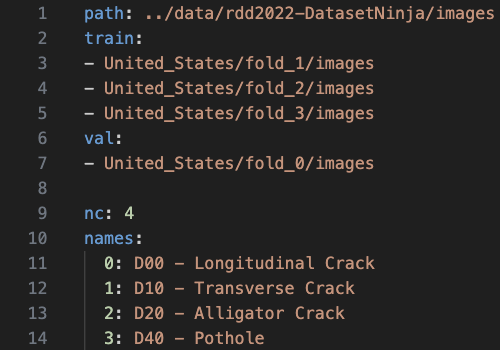
\includegraphics[width=0.5\textwidth]{img/yaml_example.png}
    \caption{Ejemplo de un fichero \textit{.yaml} que contiene la información de los datos de entrenamiento y validación para entrenar un modelo YOLO con las imágenes y anotaciones de Estados Unidos de la CRDDC2022.}
    \label{fig:yaml_example}
\end{figure}

Otra consideración importante cuando creamos los \textit{folds} es que las imágenes de una misma secuencia de imágenes, por ejemplo las imágenes de una misma calle, contienen información muy similar. Es decir, si se entrena y válida con imágenes de una misma secuencia de imágenes, se va a obtener una mejor puntuación de precisión en validación y tendremos una idea equivocada de la capacidad de generalización del modelo. La desventaja de no usar algunas secuencias de imágenes en el conjunto de entrenamiento es que el modelo no va a aprender de estas imágenes y por lo tanto va a perder información que podría ser útil para mejorar la precisión y recall del modelo. Adicionalmente, en situaciones donde el modelo se va a desplegar en producción en un lugar conocido, como por ejemplo una ciudad especifica, puede ser útil entrenar con imágenes de dicha ciudad para mejorar la precisión y recall del modelo en ese lugar. Esta compensación entre la capacidad de generalización y especialización a un entorno en concreto es un problema común en el aprendizaje automático. En este TFG se ha decidido barajar las imágenes antes de separar en \textit{folds}, ya que se considera que la ventaja de maximizar la información en cada \textit{fold} es más importante que la desventaja de que el modelo se sobre ajuste a una secuencia de imágenes. Es decir, se ha realizado un barajado (\textit{shuffle}) de las imágenes antes de separar en \textit{folds} para maximizar la información en cada \textit{fold} y de esta forma aumentar la capacidad de generalización de nuestro modelo. La desventaja es que puede que imágenes de una misma secuencia acaben en los conjuntos de entrenamiento y validación, lo que aumentara la precisión sin ser representativo de la capacidad de generalización del modelo.